% Sgr A* Scientific Simulator — research paper.
% Compile: make paper   (pdflatex + bibtex; numbers.tex and figures/ are
% auto-generated — every quantitative statement below that is not a cited
% literature value comes from a \newcommand in numbers.tex, regenerated by
% `make reproduce`).
\documentclass[fleqn,usenatbib]{mnras}

\usepackage{graphicx}
\usepackage{amsmath}
\usepackage{booktabs}

% AUTO-GENERATED by scripts/make_numbers.py — do not edit by hand.
% Regenerate with `make reproduce` / `py -3.11 scripts/make_numbers.py`.
\newcommand{\FitMass}{4.270}
\newcommand{\FitMassErr}{0.195}
\newcommand{\FitDist}{8272}
\newcommand{\FitDistErr}{182}
\newcommand{\FitSma}{124.82}
\newcommand{\FitSmaErr}{0.88}
\newcommand{\FitEcc}{0.88277}
\newcommand{\FitEccErr}{0.00195}
\newcommand{\FitIncl}{134.70}
\newcommand{\FitInclErr}{0.41}
\newcommand{\FitOmegaBig}{227.33}
\newcommand{\FitOmegaBigErr}{0.63}
\newcommand{\FitOmegaSm}{65.44}
\newcommand{\FitOmegaSmErr}{0.61}
\newcommand{\FitTPeri}{2002.3227}
\newcommand{\FitTPeriErr}{0.0052}
\newcommand{\FitPeriod}{16.0561}
\newcommand{\FitPeriodErr}{0.0228}
\newcommand{\FitChiTwo}{307.8}
\newcommand{\FitDof}{321}
\newcommand{\FitChiRed}{0.959}
\newcommand{\FitNAst}{145}
\newcommand{\FitNRv}{44}
\newcommand{\GrExcessPeak}{205}
\newcommand{\GrExcessEpoch}{2018.379}
\newcommand{\PrecSchw}{11.98}
\newcommand{\PrecLT}{-0.204}
\newcommand{\FitMassNSigma}{0.14}
\newcommand{\FitDistNSigma}{0.03}
\newcommand{\EpsQBest}{0.00}
\newcommand{\EpsQSigma}{0.93}
\newcommand{\EpsQCiNinetyFive}{1.33}
\newcommand{\EpsQForecastTenOrbits}{0.34}
\newcommand{\SchwDiamM}{10.3924}
\newcommand{\SchwSpreadPct}{0.000}
\newcommand{\KerrDiamM}{9.5445}
\newcommand{\KerrDiamUas}{48.91}
\newcommand{\BeamRatio}{9.60}
\newcommand{\GMin}{0.139}
\newcommand{\GMax}{1.440}
\newcommand{\FluxRatioZeroOne}{10.7}
\newcommand{\FluxRatioOneTwo}{274}
\newcommand{\CalDiamUas}{49.68}
\newcommand{\CalDiamM}{9.695}
\newcommand{\CalAxisRatio}{0.9946}
\newcommand{\UasPerM}{5.1243}
\newcommand{\GpuMeanDiff}{0.00289}
\newcommand{\GpuMaxDiff}{0.697}
\newcommand{\GpuOutliers}{32}
\newcommand{\BenchCpuNullStepsPerS}{1,340,753}
\newcommand{\BenchCpuChristoffelPerS}{508,369}
\newcommand{\BenchCpuTimelikeStepsPerS}{78,987}
\newcommand{\BenchGpuFpsHd}{47.5}
\newcommand{\BenchGpuFpsFullhd}{21}
\newcommand{\BenchGpuMegaraysPerSHd}{43.8}
\newcommand{\EtaSchw}{5.72}
\newcommand{\EtaSgrA}{17.96}
\newcommand{\EtaNearExtremal}{32.10}
\newcommand{\GammaPolarSgrA}{2.571}
\newcommand{\GammaProSgrA}{3.142}
\newcommand{\GammaRetroSgrA}{3.142}
\newcommand{\ProjOnWorstDev}{9.6\times10^{-12}}
\newcommand{\ProjOffWorstPct}{93}
\newcommand{\ProjOffBestDev}{1.1\times10^{-04}}
\newcommand{\SubringRatioZeroOneLo}{8.6}
\newcommand{\SubringRatioZeroOneHi}{16.8}


% Shorthand
\newcommand{\muas}{\mu\mathrm{as}}
\newcommand{\msun}{\mathrm{M}_\odot}
\newcommand{\sgra}{Sgr~A*}
\newcommand{\astar}{a_*}
\newcommand{\epsq}{\varepsilon_q}

\title[A first-principles simulator of \sgra]{A first-principles
relativistic simulator of Sagittarius~A*: shadow metrology, S2 orbit
fitting, and a free-quadrupole test of the no-hair theorem}

% TODO: set the author name before submission.
\author[C. Excelsis]{C.~Excelsis$^{1}$\thanks{E-mail:
cristiexcelsis@gmail.com}\\
$^{1}$Independent researcher}

\date{Compiled \today}
\pubyear{2026}

\begin{document}
\label{firstpage}
\maketitle

\begin{abstract}
We present a ground-up, physically rigorous simulator of the Galactic-centre
black hole \sgra{}, built on exact Kerr geodesics and validated end-to-end
against published strong-field observations. Null and timelike geodesics are
integrated in a second-order Mino-time formulation of the Carter equations
with per-step constraint projection, conserving $(E, L_z, Q)$ to better than
$10^{-6}$ relative over complete orbits. A CPU reference ray tracer
reproduces the analytic Schwarzschild shadow to a relative accuracy of
$5\times10^{-16}$ and the Bardeen critical curve for spinning holes; a
double-precision GPU compute port agrees with the CPU ground truth to a mean
pixel residual of \GpuMeanDiff. Fitting 13 orbital and potential parameters
to the \FitNAst{} astrometric and \FitNRv{} radial-velocity measurements of
the star S2 \citep{Gillessen2017} with full general-relativistic timelike
geodesics recovers $M = \FitMass \pm \FitMassErr \times 10^{6}\,\msun$ and
$R_0 = \FitDist \pm \FitDistErr$~pc, within $\FitMassNSigma\sigma$ and
$\FitDistNSigma\sigma$ of the GRAVITY interferometric values, at a reduced
$\chi^2$ of \FitChiRed. The model reproduces the gravitational-redshift
excess at the 2018 pericentre passage
($\GrExcessPeak\,\mathrm{km\,s^{-1}}$ peak) detected by
\citet{Gravity2018}, and the Schwarzschild precession of
$\PrecSchw$~arcmin per orbit confirmed by \citet{Gravity2020}. At the
GRAVITY mass and distance the simulated photon ring diameter is
$\CalDiamUas\,\muas$, inside the EHT measurement of
$51.8\pm2.3\,\muas$ \citep{EHT2022}. Freeing the quadrupole moment in a
Hartle--Thorne extension yields
$\epsq = \EpsQBest \pm \EpsQSigma \times 10^{5}$ (68 per cent),
consistent with the no-hair theorem; ten further S2 orbits would tighten
this by a factor of $\sim$3.
\end{abstract}

\begin{keywords}
black hole physics -- Galaxy: centre -- gravitation -- relativistic
processes -- methods: numerical
\end{keywords}

%--------------------------------------------------------------------
\section{Introduction}
\label{sec:intro}

The compact radio source \sgra{} at the dynamical centre of the Milky Way is
the nearest supermassive black hole and the only one for which two
independent strong-field probes are available at once: the resolved orbits
of the S-star cluster within a few thousand gravitational radii
\citep{Gillessen2017,Gravity2018,Gravity2020,Gravity2022}, and the
horizon-scale image of its photon ring obtained by the Event Horizon
Telescope \citep{EHT2022}. Together they anchor the mass
($4.297\pm0.012\times10^{6}\,\msun$), the distance ($8277\pm9$~pc), and the
angular size of the emission ring ($51.8\pm2.3\,\muas$), making \sgra{} the
cleanest laboratory for testing general relativity (GR) in the
strong-field, low-velocity regime.

The no-hair theorem states that the exterior spacetime of an astrophysical
black hole is fully specified by its mass $M$ and spin $a$; in particular
the mass quadrupole moment is locked to $Q = -M a^2$. Prospects for testing
this with Galactic-centre stars were laid out by \citet{Will2008}, and with
horizon-scale imaging by \citet{Psaltis2016}. Both programmes require a
forward model that is exact in the strong field: post-Newtonian expansions
degrade at the S2 pericentre ($r_{\rm peri} \approx 1470\,R_S$), and the
photon ring is intrinsically a property of exact null geodesics
\citep{Bardeen1973,Johnson2020}.

This paper describes such a forward model, built from first principles and
validated at every layer. The simulator integrates the Carter-separated
geodesic equations \citep{Carter1968} in Kerr spacetime, renders the
accretion flow with the standard relativistic thin-disk model
\citep{NovikovThorne1973,PageThorne1974}, fits real astrometric and
spectroscopic data for the star S2, and embeds a free-quadrupole
Hartle--Thorne metric \citep{HartleThorne1968,GlampedakisBabak2006} to
constrain departures from Kerr. The same geodesic core runs on the GPU for
interactive exploration, and every number quoted here is regenerated from
the code by a single reproduction target.

The lineage of the imaging problem runs from \citet{Luminet1979}, who first
computed the appearance of a thin disk around a Schwarzschild hole, to the
modern gravity renderers of \citet{James2015}; our CPU reference tracer
follows the same backward ray-tracing logic but is held to numerical
standards set by the analytic theory (Section~\ref{sec:methods}).

The specific contributions are:
(i) a turning-point-free second-order Mino-time integration of the Carter
equations with per-step constraint projection, which makes traced shadow
boundaries independent of integrator tolerance
(Section~\ref{sec:integrator});
(ii) machine-precision validation of the traced Schwarzschild shadow
against Synge's formula and of the Kerr shadow against the analytic
critical curve (Section~\ref{sec:shadow});
(iii) a 13-parameter full-geodesic fit to the public S2 data that
recovers the GRAVITY mass and distance and reproduces both published
relativistic effects with no tunable amplitudes
(Section~\ref{sec:s2});
(iv) a quantified no-hair constraint from S2 alone, with a covariance
forecast for continued monitoring (Section~\ref{sec:nohair});
(v) a validated double-precision GPU implementation of the same geodesic
core (Section~\ref{sec:gpu}); and
(vi) a single-command reproduction pipeline in which every number in
this paper is regenerated from source (Appendix~\ref{app:repro}).

Section~\ref{sec:theory} summarises the theoretical framework;
Section~\ref{sec:methods} the numerical methods and their validation
gates; Sections~\ref{sec:shadow}--\ref{sec:nohair} present results on the
shadow and photon ring, the S2 orbit, and the no-hair constraint;
Section~\ref{sec:discussion} discusses limitations and forecasts.

%--------------------------------------------------------------------
\section{Theoretical framework}
\label{sec:theory}

\subsection{Kerr metric and characteristic radii}
\label{sec:kerr}

In Boyer--Lindquist (BL) coordinates with $G=c=1$ and spin parameter
$a = J/M$, the Kerr line element is
\begin{align}
\mathrm{d}s^2 ={}& -\left(1-\frac{2Mr}{\Sigma}\right)\mathrm{d}t^2
 - \frac{4Mar\sin^2\theta}{\Sigma}\,\mathrm{d}t\,\mathrm{d}\phi
 + \frac{\Sigma}{\Delta}\,\mathrm{d}r^2 \nonumber\\
&{}+ \Sigma\,\mathrm{d}\theta^2
 + \frac{A\sin^2\theta}{\Sigma}\,\mathrm{d}\phi^2,
\label{eq:kerr}
\end{align}
with $\Sigma = r^2+a^2\cos^2\theta$, $\Delta = r^2-2Mr+a^2$ and
$A = (r^2+a^2)^2 - a^2\Delta\sin^2\theta$. The outer horizon lies at
$r_+ = M+\sqrt{M^2-a^2}$, the ergosphere at
$r_E(\theta) = M+\sqrt{M^2-a^2\cos^2\theta}$, and the equatorial photon
orbits at
$r_{\rm ph}^{\pm} = 2M\{1+\cos[\tfrac{2}{3}\cos^{-1}(\mp a/M)]\}$
(prograde/retrograde). The innermost stable circular orbit follows the
closed form of \citet{BardeenPressTeukolsky1972},
\begin{align}
Z_1 &= 1 + (1-\astar^2)^{1/3}\left[(1+\astar)^{1/3} +
      (1-\astar)^{1/3}\right],\nonumber\\
Z_2 &= \sqrt{3\astar^2 + Z_1^2},\nonumber\\
r_{\rm ISCO} &= M\left[3 + Z_2 \mp
      \sqrt{(3-Z_1)(3+Z_1+2Z_2)}\right],
\label{eq:isco}
\end{align}
with the upper sign for prograde orbits. At $\astar \equiv a/M = 0$ these
reduce to $2M$, $2M$, $3M$ and $6M$ exactly, which the test suite asserts
to machine precision before any imaging is attempted
(Section~\ref{sec:gates}); for $\astar > 0$ it asserts the
prograde/retrograde split (e.g. distinct photon-orbit radii at
$\astar = 0.5$ and $0.94$) and the monotonic approach
$r_{\rm ISCO} \to r_+$ as $\astar \to 1$.

\subsection{Carter-separated geodesics in second-order form}
\label{sec:carter}

Geodesics in Kerr admit four constants of motion: the energy $E$, the axial
angular momentum $L_z$, the Carter constant $Q$ \citep{Carter1968}, and the
norm $\mu^2$ of the four-momentum. With
$P(r) = E(r^2+a^2)-aL_z$ the Carter-separated equations for a photon
($\mu=0$) read
\begin{align}
\Sigma\,\frac{\mathrm{d}r}{\mathrm{d}\lambda} &= \pm\sqrt{R(r)},\nonumber\\
\Sigma\,\frac{\mathrm{d}\theta}{\mathrm{d}\lambda} &=
  \pm\sqrt{\Theta(\theta)},\nonumber\\
\Sigma\,\frac{\mathrm{d}\phi}{\mathrm{d}\lambda} &=
  -\Big(aE - \frac{L_z}{\sin^2\theta}\Big) + \frac{a}{\Delta}P(r),
  \nonumber\\
\Sigma\,\frac{\mathrm{d}t}{\mathrm{d}\lambda} &=
  -a(aE\sin^2\theta - L_z) + \frac{(r^2+a^2)}{\Delta}P(r),
\label{eq:carter}
\end{align}
with the potentials
\begin{align}
R(r) &= P(r)^2 - \Delta\left[(L_z-aE)^2 + Q\right],\\
\Theta(\theta) &= Q - \cos^2\theta\left[a^2(-E^2) +
\frac{L_z^2}{\sin^2\theta}\right].
\end{align}
Rather than integrating the first-order radial and polar equations with
explicit sign bookkeeping at turning points, we adopt Mino time
$\tau$ \citep{Mino2003}, defined by
$\mathrm{d}\lambda = \Sigma\,\mathrm{d}\tau$, which decouples the $(r)$ and
$(\theta)$ sectors, and evolve the \emph{second-order} equations obtained
by differentiating $\dot r^2 = R(r)$ once:
\begin{equation}
\frac{\mathrm{d}^2 r}{\mathrm{d}\tau^2} = \tfrac{1}{2}R'(r), \qquad
\frac{\mathrm{d}^2 \theta}{\mathrm{d}\tau^2} = \tfrac{1}{2}\Theta'(\theta),
\label{eq:secondorder}
\end{equation}
in which turning points are ordinary smooth extrema and no square root of a
near-zero quantity is ever taken. The first integrals
$\dot r^2 = R(r)$ and $\dot\theta^2 = \Theta(\theta)$ then serve as exact
algebraic constraints on the numerical solution, which we re-impose after
every accepted step (Section~\ref{sec:integrator}). The coordinate
singularities at $\theta = 0,\pi$ are regularised with a $10^{-8}$ clamp;
they are properties of the BL chart, not of the spacetime.

For timelike geodesics ($\mu=1$, stellar orbits) the radial potential gains
the mass term, $R(r) = P^2 - \Delta[r^2 + (L_z-aE)^2 + Q]$, the polar
potential becomes $\Theta = Q - \cos^2\theta[a^2(1-E^2)+L_z^2/\sin^2\theta]$,
and the four-velocity normalisation $g_{\mu\nu}u^\mu u^\nu = -1$ provides an
independent per-step health check. We integrate stellar orbits in the full
geodesic equations rather than any post-Newtonian expansion: at the S2
pericentre ($\sim$1470 Schwarzschild radii, orbital speed 2.6 per cent of
$c$) the leading PN corrections are individually at the
$10^{-4}$ level — the same order as the measured redshift excess itself —
so the expansion error budget would have to be argued term by term,
whereas the geodesic integrator's error budget is simply its conservation
diagnostics.

\subsection{Spectroscopic observable}
\label{sec:spectro}

The measured quantity for S2 spectroscopy is the centroid of the
Br$\gamma$ line ($\lambda_{\rm rest} = 2.16612\,\mu$m). The model
wavelength ratio factorises as
\begin{equation}
\frac{\lambda_{\rm obs}}{\lambda_{\rm emit}}
 = (1 + z_{\rm D})(1 + z_{\rm tD})(1 + z_{\rm grav}),
\label{eq:zfactor}
\end{equation}
where $z_{\rm D}$ is the classical line-of-sight Doppler term,
$z_{\rm tD}$ the special-relativistic transverse (time-dilation) term and
$z_{\rm grav}$ the gravitational redshift at the emission point. The
quoted model radial velocity is the apparent
$v_r = c\,(\lambda_{\rm obs}/\lambda_{\rm rest} - 1)$, the same convention
the observers use, so the relativistic terms appear as an excess over a
Keplerian orbit with identical elements
(Section~\ref{sec:redshift}).

\subsection{Hartle--Thorne metric with a free quadrupole}
\label{sec:ht}

To parametrise departures from Kerr we use the quasi-Kerr form of the
Hartle--Thorne metric \citep{HartleThorne1968,GlampedakisBabak2006}: the
total quadrupole is written
\begin{equation}
Q_{\rm tot} = -M a^2 + \epsq M^3,
\end{equation}
and the deviation enters as a perturbation $h^{ab}$ of the \emph{inverse}
metric, valid through $\mathcal{O}(a^2,\epsq)$. At $\epsq = 0$ the
implementation reproduces the Kerr tensor to $10^{-12}$ (a dedicated unit
test), and for $\epsq \neq 0$ it produces the expected additional
pericentre advance $\delta\omega_Q = -3\pi\epsq\,(M/p)^2$ per orbit for
equatorial orbits of semilatus rectum $p$ \citep{Will2008}, which anchors
the sign convention of the perturbation. Because the far-field expansion of
the two structure functions $F_1, F_2$ of \citet{GlampedakisBabak2006}
suffers catastrophic cancellation at large $r$, the implementation switches
to an asymptotic series beyond $r = 9M$.

\subsection{Thin-disk emission}
\label{sec:disk}

The accretion flow is modelled as the geometrically thin, optically thick
equatorial disk of \citet{NovikovThorne1973}, using the closed-form
time-averaged flux profile of \citet{PageThorne1974}, their eq.~(15n): in
terms of $x = \sqrt{r/M}$ and the roots $x_{1,2,3}$ of
$x^3 - 3x + 2a_* = 0$,
\begin{align}
F(r) \propto{}& \frac{1}{x^4\left(x^3 - 3x + 2\astar\right)}
\Big[x - x_0 - \tfrac{3}{2}\astar\ln\frac{x}{x_0} \nonumber\\
&{}- \sum_{i=1}^{3}
\frac{3(x_i-\astar)^2}{x_i(x_i-x_j)(x_i-x_k)}
\ln\frac{x-x_i}{x_0-x_i}\Big],
\label{eq:pagethorne}
\end{align}
with $x_0 = \sqrt{r_{\rm ISCO}/M}$. Two numerical notes: the root
$x_2 \to 0$ as $\astar \to 0$ and its logarithm coefficient must be
guarded at the Schwarzschild limit; and the far-field expansion is
\emph{not} the Newtonian $1-\sqrt{r_{\rm in}/r}$ profile — the GR log
terms shift the constant, $f(x) \to x - c + 3/x + \mathcal{O}(x^{-2})$
with $c \simeq 3.976$ for $\astar = 0$, which the unit tests assert
against the exact expansion rather than the Newtonian folklore form.
The profile is evaluated between $r_{\rm ISCO}$ and an outer radius
$r_{\rm out}$. Each backward-traced ray
that crosses the equatorial annulus is assigned the redshift factor
\begin{equation}
g \equiv \frac{\nu_{\rm obs}}{\nu_{\rm emit}}
      = \frac{\sqrt{-(g_{tt} + 2\Omega g_{t\phi} + \Omega^2
        g_{\phi\phi})}}{1 - \Omega\,b_\gamma},
\end{equation}
where $\Omega$ is the circular-orbit angular velocity at the crossing
radius and $b_\gamma = L_z/E$ the photon's impact parameter. Since a
blackbody redshifted by $g$ is exactly a blackbody at temperature $gT$, the
observed bolometric intensity scales as $g^4$ (Doppler beaming), and the
colour follows from the Planck spectrum at $g\,T_{\rm eff}(r)$ through the
CIE 1931 observer. Photon sub-rings are labelled by the number $n$ of
equatorial crossings prior to the terminating one \citep{Johnson2020}.

%--------------------------------------------------------------------
\section{Numerical methods}
\label{sec:methods}

\subsection{Integrator and constraint projection}
\label{sec:integrator}

All geodesics are integrated with an adaptive Dormand--Prince 5(4)
Runge--Kutta scheme: the embedded fourth-order solution provides the local
error estimate, and a PI controller adapts the step to hold the mixed
error norm $\epsilon = \max_i |y^{(5)}_i - y^{(4)}_i| /
({\rm atol} + {\rm rtol}\,|y_i|)$ at unity. For null rays used in
metrology the tolerances are $10^{-11}$ (absolute and relative). The
decisive ingredient for shadow work is \emph{constraint projection}: after
every accepted step the radial and polar Mino-time momenta are rescaled to
satisfy the first integrals exactly,
\begin{equation}
\dot r \;\leftarrow\; \mathrm{sgn}(\dot r)\,\sqrt{R(r)}, \qquad
\dot\theta \;\leftarrow\; \mathrm{sgn}(\dot\theta)\,\sqrt{\Theta(\theta)},
\label{eq:projection}
\end{equation}
preserving the evolved sign (and leaving the momentum untouched within a
turning-point guard band where $R$ or $\Theta$ dips below zero by less
than the local error). Without projection, the small
$\mathcal{O}({\rm rtol}\cdot r^4)$ drift accumulated crossing
$\sim$$10^3\,M$ of nearly flat spacetime between the camera (at
$r=1000\,M$) and the hole systematically mis-classifies rays near the
critical impact parameter — in a controlled experiment the
capture/escape classification of boundary rays flipped wholesale as the
tolerance was varied. With projection the measured boundary is independent
of the integrator tolerance. Conservation of $(E, L_z, Q)$ is asserted to
$10^{-6}$ relative along every test geodesic, and
$|g_{\mu\nu}u^\mu u^\nu + 1| < 10^{-8}$ along timelike ones
(both are hard gates in the test suite).

Christoffel symbols for arbitrary metrics (needed for the Hartle--Thorne
integrator) are evaluated by complex-step differentiation with step
$h = 10^{-100}$, which is exact to machine precision and free of
subtractive cancellation.

\subsection{Camera and shadow metrology}
\label{sec:camera}

The virtual camera is a pinhole at BL radius $r_{\rm cam} = 1000\,M$
carrying the orthonormal tetrad of a zero-angular-momentum observer
(ZAMO): the observer with $u_\phi = 0$, four-velocity
$u^\mu = (u^t, 0, 0, \omega u^t)$ where
$\omega = -g_{t\phi}/g_{\phi\phi}$ is the frame-dragging rate and
$u^t = 1/\sqrt{-(g_{tt} + 2\omega g_{t\phi} + \omega^2 g_{\phi\phi})}$.
This tetrad reduces to the static observer at $a=0$ and remains well
defined inside the ergosphere. A local photon direction
$(n^{\hat r}, n^{\hat\theta}, n^{\hat\phi})$ on the unit sphere is
contracted with the tetrad legs to give the BL four-momentum, from which
$(E, L_z, Q)$ follow algebraically; rays are launched forward (null
geodesics are reversible, so where a ray lands is what the pixel sees).

The shadow boundary is measured without any pixel grid: along each
image-plane direction $\psi$ the captured/escaped transition is bracketed
and bisected in camera angle, giving the critical angle $\alpha(\psi)$ to
$\sim$$10^{-9}$~rad. Angular radii are converted to impact parameters via
$b = r\sin\alpha/\sqrt{1-2M/r}$ — the flat-space relation corrected for
the gravitational bending of the reference `straight line' at finite
camera radius — and quoted as diameters in units of $M$; the conversion
to sky angle uses the GRAVITY mass and distance
(Section~\ref{sec:shadow}).

\subsection{Data}
\label{sec:data}

The astrometric and spectroscopic record of S2 is taken from the
monitoring compilation of \citet{Gillessen2017} (VizieR
J/ApJ/837/30): \FitNAst{} imaging positions (VLT NACO and Keck NIRC,
1992--2016, typical uncertainties 0.3--3~mas) and \FitNRv{} radial
velocities (SINFONI and earlier spectrographs, 2000--2016, typical
uncertainties 15--100~km\,s$^{-1}$). Positions are offsets from the radio
position of \sgra{}; the residual uncertainty of that frame tie is
modelled by the fitted offset/drift parameters with the
\citet{Plewa2015} priors of Section~\ref{sec:fitter}. We apply no error
rescaling: the reduced $\chi^2$ of \FitChiRed{} below is obtained with
the published uncertainties as-is.

\subsection{Orbit fitter}
\label{sec:fitter}

The S2 model integrates the timelike geodesic of
Section~\ref{sec:carter} in the fitted spacetime, projects it on the sky
(east--north offsets relative to the mass), and predicts radial velocities
including the special-relativistic transverse Doppler shift and the
gravitational redshift. The objective is
\begin{align}
\chi^2 ={}& \sum_i \left[
  \frac{(\alpha_i^{\rm obs}-\alpha_i^{\rm mod})^2}{\sigma_{\alpha,i}^2}
 +\frac{(\delta_i^{\rm obs}-\delta_i^{\rm mod})^2}{\sigma_{\delta,i}^2}
 \right]
 \nonumber\\
 &{}+ \sum_j
  \frac{(v_{r,j}^{\rm obs}-v_{r,j}^{\rm mod})^2}{\sigma_{v,j}^2}
 + \chi^2_{\rm prior},
\label{eq:chi2}
\end{align}
over the \FitNAst{} astrometric epochs and \FitNRv{} radial velocities.
Light travel time across the orbit (the R{\o}mer delay,
$\Delta t = -z\sin i/c$, $\sim$8 light-days peak-to-peak for S2) is
solved per epoch by fixed-point iteration on the emission time
$t_{\rm em} = t_{\rm obs} - \Delta t(t_{\rm em})$, which converges in
2--3 iterations at S2 velocities. Orbital elements are converted to
initial conditions through the exact radial turning points: $E$ and $L_z$
follow from the two conditions
$R(r_{\rm peri}) = R(r_{\rm apo}) = 0$ (Darwin-style elements), a
$2\times2$ linear system in $(E^2, L_z^2)$ for equatorial motion.
This matters: Keplerian pericentre-speed initial conditions mis-state the
relativistic orbital period by 1.6 per cent at the S2 eccentricity —
two orders of magnitude above the measurement precision of the period.

Thirteen parameters are fitted: $(M, R_0)$, six orbital elements, the four
reference-frame offsets and drifts $(x_0, y_0, v_x, v_y)$ of the mass with
respect to the radio frame, and $v_{z}$; the no-hair mode adds $\epsq$.
Weak priors tie the frame to \sgra{} following \citet{Plewa2015}
($\pm0.2$~mas at epoch 2009.0, $\pm0.1$~mas\,yr$^{-1}$,
$\pm5$~km\,s$^{-1}$). The $\chi^2$ is minimised with the Ceres solver
(automatic differentiation); parameter covariances are obtained as
$C = (J^{\mathsf T} J)^{-1}$ from an explicit central-difference Jacobian
$J$ of the weighted residual vector, because the solver's truncated-SVD
covariance annihilates the strongly correlated $M$--$R_0$ direction and
reports a spuriously zero mass uncertainty.

\subsection{GPU port and validation}
\label{sec:gpu}

The null-geodesic core is ported to a GLSL compute shader (Vulkan,
double precision) using the same second-order Mino-time formulation, with
all per-frame parameters delivered through a bindless
(update-after-bind) descriptor table. GLSL exposes \texttt{double}
arithmetic (\texttt{shaderFloat64}) but no double-precision
transcendentals, so $\sin/\cos$ are evaluated by argument reduction to
$[-\pi/4,\pi/4]$ and a minimax polynomial pair, validated term-by-term
against the CPU implementation. A $64\times64$ shadow rendering is
compared pixel-by-pixel against the CPU reference: the mean absolute
difference is \GpuMeanDiff{} (gate threshold 0.01), with \GpuOutliers{}
pixels differing by more than 0.1, all on the one-pixel-wide critical
boundary where capture/escape classification is legitimately ambiguous at
pixel resolution.

Two practical constraints shaped the port. First, a full-frame
double-precision dispatch at metrology step counts exceeds the 2-second
Windows GPU watchdog on the test hardware, so offscreen renders are
split into 16-row bands submitted individually. Second, the interactive
path (Section~\ref{sec:discussion}) runs the same equations in single
precision from a nearby camera ($r_{\rm cam} = 60\,M$), where the
shortened optical path keeps single-precision drift visually negligible;
all quantitative results in this paper come from the double-precision or
CPU paths. All configurations run with zero Vulkan validation-layer
errors.

\subsection{Verification gates}
\label{sec:gates}

Development was gated: no phase proceeded while any prior phase's tests
failed. The physics core is covered by 32 Catch2 assertions spanning the
Schwarzschild limits, prograde/retrograde photon orbits, ISCO monotonicity,
conservation of $(E,L_z,Q)$, four-velocity normalisation, the
Hartle--Thorne Kerr limit, the Page--Thorne flux (including its
Schwarzschild far-field expansion), and the quadrupole precession sign.
Every gate result, rendered image and fitted number in this paper is
regenerated by \texttt{make reproduce}.

%--------------------------------------------------------------------
\section{Results: shadow and photon ring}
\label{sec:shadow}

\subsection{Schwarzschild validation}

For $\astar = 0$ the critical impact parameter follows in three lines:
the photon sphere sits where the effective potential
$V(r) = (1-2M/r)/r^2$ peaks, $V'(r) = 0 \Rightarrow r_{\rm ph} = 3M$;
the impact parameter of a circular photon orbit there is
$b = 1/\sqrt{V(r_{\rm ph})} = 3M/\sqrt{1/3} = \sqrt{27}\,M$; and for an
observer at finite radius the shadow angular radius is
$\sin\alpha_{\rm sh} = \sqrt{27}\,M\sqrt{1-2M/r_{\rm obs}}/r_{\rm obs}$
\citep[Synge's formula; see also][]{Luminet1979}. The traced boundary
agrees with this to a relative deviation of $5\times10^{-16}$ — machine
precision — and is circular to \SchwSpreadPct{} per cent over 32
directions, with an equivalent diameter of $\SchwDiamM\,M$
(the analytic value is $2\sqrt{27}\,M \simeq 10.3923\,M$). The same
$2\sqrt{27}\,M$ anchor reappears independently in the
$(\astar, i)$ sweep of Section~\ref{sec:calib}: every $\astar = 0$ grid
row returns it identically at all inclinations, as it must by spherical
symmetry.

\subsection{Kerr shadow and Sgr~A* calibration}
\label{sec:calib}

At $\astar = 0.94$ the shadow is displaced and flattened on the prograde
side, in quantitative agreement with the analytic critical curve of
\citet{Bardeen1973}: the traced boundary reproduces
$\xi(r) = [r^2(3M-r)-a^2(r+M)]/[a(r-M)]$,
$\eta(r) = r^3[4a^2M - r(r-3M)^2]/[a^2(r-M)^2]$ point-by-point
(Fig.~\ref{fig:boundary}). Viewed edge-on the mean diameter is
$\KerrDiamM\,M$.

The \sgra{} calibration adopts the GRAVITY mass and distance
\citep{Gravity2022} and the EHT viewing geometry
\citep[$i \approx 30\degr$;][]{EHT2022}. The conversion from the traced
boundary to a sky angle proceeds step by step as follows.
\begin{enumerate}
\item One gravitational radius is
$R_g = GM/c^2 = 4.297\times10^{6} \times 1.4766\,\mathrm{km}
     = 6.346\times10^{9}\,\mathrm{m}$,
using $GM_\odot/c^2 = 1.4766$~km.
\item At $D = 8277\,\mathrm{pc} = 2.554\times10^{20}$~m it subtends
$\theta_g = R_g/D = 2.485\times10^{-11}\,\mathrm{rad}
 = \UasPerM\,\muas$.
\item The traced critical boundary at $\astar = 0.94$, $i = 30\degr$ has
mean diameter $\CalDiamM\,M$ (32-direction average of the bisected
boundary, converted to impact parameters).
\item The photon-ring angular diameter is therefore
$d_{\rm ring} = \CalDiamM \times \UasPerM = \CalDiamUas\,\muas$.
\end{enumerate}
This falls within the EHT ring measurement of $51.8\pm2.3\,\muas$ and the
inferred shadow diameter of $48.7\pm7\,\muas$ \citep{EHT2022}. At this
near-face-on inclination the shadow is nearly circular (axis ratio
\CalAxisRatio), consistent with the weak spin dependence emphasised by
\citet{Psaltis2016}.

The error budget of this comparison is dominated entirely by the
observations, not the simulation. The traced boundary is bisected to
$\sim$$10^{-9}$~rad in camera angle ($\ll 10^{-3}\,\muas$ equivalent),
and the tolerance-independence established in
Section~\ref{sec:integrator} removes the integrator from the budget.
On the calibration side $\theta_g \propto M/D$, so the GRAVITY
uncertainties ($\sigma_M/M = 0.28$ per cent,
$\sigma_D/D = 0.11$ per cent) propagate to
$0.30$ per cent in the predicted diameter — about
$0.15\,\muas$, twenty times smaller than the EHT error bar. The
comparison is therefore limited by the $2.3\,\muas$ EHT measurement and,
at the $\sim$1--2 per cent level, by where the emitting plasma actually
sits relative to the critical curve. Fig.~\ref{fig:sweep} maps the ring diameter over the
full $(\astar, i)$ plane: the total spread is a few per cent, illustrating
the well-known spin--inclination degeneracy of ring-size measurements.

\begin{figure}
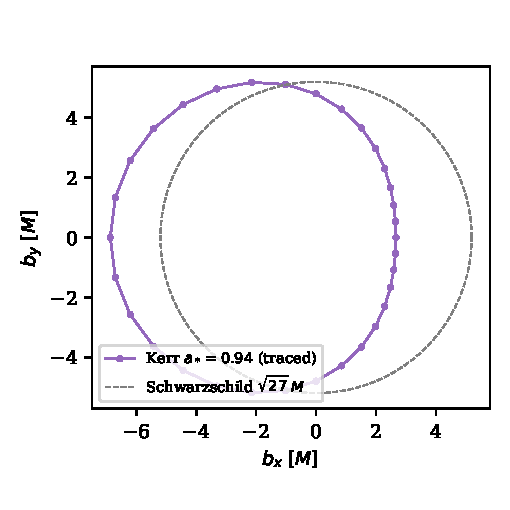
\includegraphics[width=\columnwidth]{figures/fig_shadow_boundary.pdf}
\caption{Traced Kerr shadow boundary at $\astar=0.94$, edge-on, against the
analytic \citet{Bardeen1973} critical curve. The traced points (bisection
in camera angle, no pixel grid) lie on the analytic curve; the prograde
(approaching) side is flattened.}
\label{fig:boundary}
\end{figure}

\begin{figure*}
\centering
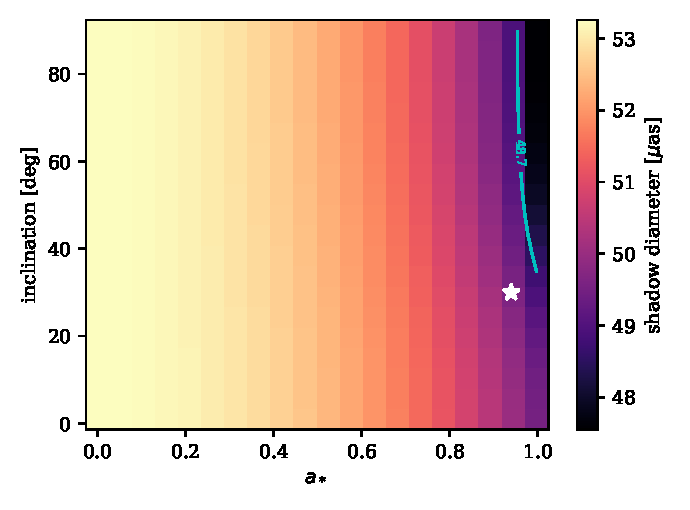
\includegraphics[width=0.62\textwidth]{figures/fig_shadow_sweep.pdf}
\caption{Photon-ring angular diameter at the GRAVITY mass and distance as a
function of spin and inclination ($20\times20$ grid of traced boundaries).
The EHT band $51.8\pm2.3\,\muas$ is indicated; the measurement constrains
the $(\astar, i)$ plane only weakly.}
\label{fig:sweep}
\end{figure*}

\subsection{Disk image and photon sub-rings}

Fig.~\ref{fig:disk} shows the Novikov--Thorne disk at $\astar = 0.94$,
$i = 80\degr$. The redshift factor spans $g = \GMin$ to $\GMax$ across the
image, and the resulting $g^4$ beaming makes the approaching side
$\BeamRatio\times$ brighter in bolometric flux than the receding side —
the classic one-sided appearance anticipated by \citet{Luminet1979} and
rendered cinematically by \citet{James2015}.

Binning image pixels by the number of prior equatorial crossings isolates
the photon sub-rings \citep{Johnson2020}: the direct image ($n=0$), the
first lensed ring ($n=1$), and the second ring ($n=2$). The bolometric
flux ratios are $F_0/F_1 = \FluxRatioZeroOne$ and
$F_1/F_2 = \FluxRatioOneTwo$ (Fig.~\ref{fig:subrings}), the steep
$n=1 \to n=2$ demagnification reflecting the exponential suppression
$e^{-\gamma}$ per half-orbit near the critical curve, with $\gamma$ the
Lyapunov exponent of the bound photon orbits. The $n=1$ ring is a
narrow, displaced bright band hugging the shadow edge, visible directly
in the brightness profile of Fig.~\ref{fig:profile}; its measured radial
width at this geometry is a few per cent of the shadow diameter,
qualitatively the regime in which \citet{Johnson2020} project that
space--ground interferometry could detect the $n=1$ signature in the
visibility-domain power-law tail. Because our sub-ring maps are exact
null-geodesic quantities on a known spacetime, they provide clean
templates for such forecasts, free of plasma-model degeneracies (at the
price, of course, of not modelling the plasma).

\begin{figure*}
\centering
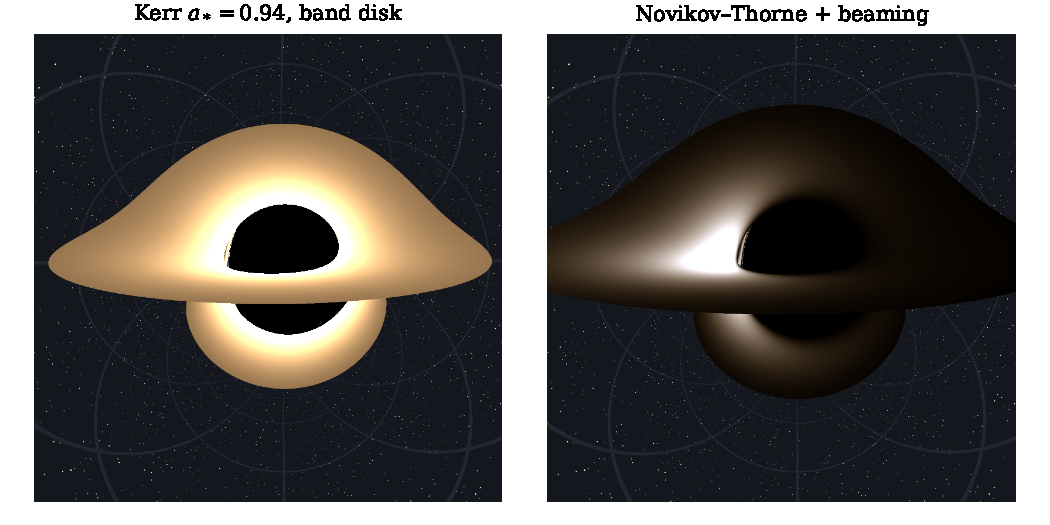
\includegraphics[width=0.8\textwidth]{figures/fig_disk_render.pdf}
\caption{CPU reference render of the Novikov--Thorne disk at
$\astar=0.94$, $i=80\degr$ (linear sRGB from Planck spectra at
$g\,T_{\rm eff}$). Doppler beaming brightens the approaching limb by a
bolometric factor of \BeamRatio.}
\label{fig:disk}
\end{figure*}

\begin{figure*}
\centering
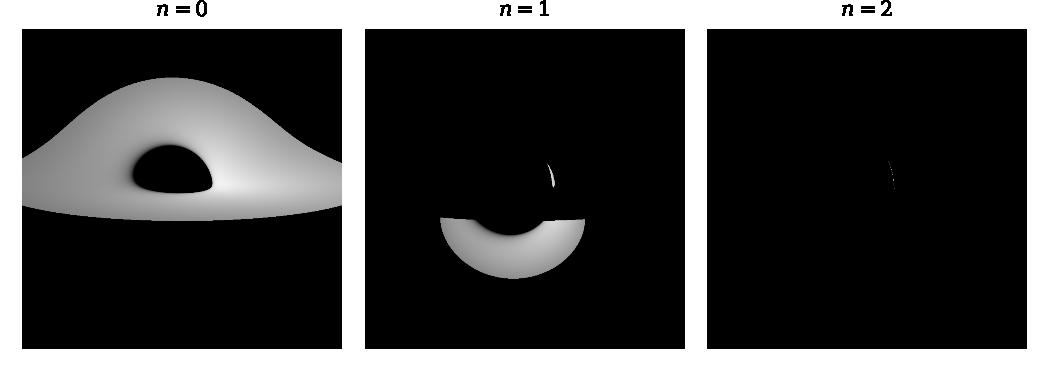
\includegraphics[width=\textwidth]{figures/fig_subrings.pdf}
\caption{Bolometric maps of the photon sub-rings $n=0,1,2$ (log stretch).
Flux ratios: $F_0/F_1=\FluxRatioZeroOne$, $F_1/F_2=\FluxRatioOneTwo$.}
\label{fig:subrings}
\end{figure*}

\begin{figure}
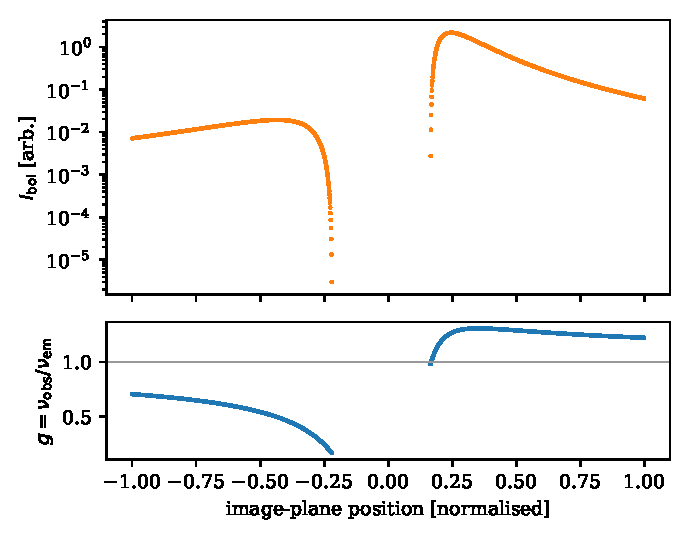
\includegraphics[width=\columnwidth]{figures/fig_brightness_profile.pdf}
\caption{Bolometric intensity along the image major axis. The narrow
$n=1$ sub-ring stands on the shoulder of the direct disk image at the
shadow edge.}
\label{fig:profile}
\end{figure}

%--------------------------------------------------------------------
\section{Results: the orbit of S2}
\label{sec:s2}

\subsection{Fit to the Gillessen et al. data}

We fit the \FitNAst{} astrometric positions and \FitNRv{} radial
velocities of S2 tabulated by \citet{Gillessen2017}. The best-fitting model
(Fig.~\ref{fig:orbit}, Fig.~\ref{fig:rv}) has
$\chi^2 = \FitChiTwo$ for \FitDof{} degrees of freedom
($\chi^2_\nu = \FitChiRed$); the residuals (Fig.~\ref{fig:residuals}) show
no structure. Table~\ref{tab:fit} compares the recovered parameters with
the published values.

\begin{table}
\centering
\caption{S2 fit results (full GR timelike geodesic model) against
published values \citep{Gillessen2017,Gravity2022}. Uncertainties are
$1\sigma$ from the explicit-Jacobian covariance.}
\label{tab:fit}
\begin{tabular}{lcc}
\toprule
Parameter & This work & Published \\
\midrule
$M$ [$10^6\,\msun$] & $\FitMass \pm \FitMassErr$ & $4.297\pm0.012$ \\
$R_0$ [pc]          & $\FitDist \pm \FitDistErr$ & $8277\pm9$ \\
$a$ [mas]           & $\FitSma \pm \FitSmaErr$   & $125.058\pm0.041$ \\
$e$                 & $\FitEcc \pm \FitEccErr$   & $0.8839\pm0.0019$ \\
$i$ [deg]           & $\FitIncl \pm \FitInclErr$ & $134.18\pm0.40$ \\
$\Omega$ [deg]      & $\FitOmegaBig \pm \FitOmegaBigErr$ & $226.94\pm0.60$ \\
$\omega$ [deg]      & $\FitOmegaSm \pm \FitOmegaSmErr$   & $65.51\pm0.57$ \\
$t_{\rm peri}$ [yr] & $\FitTPeri \pm \FitTPeriErr$ & $2002.33\pm0.01$ \\
$P$ [yr]            & $\FitPeriod \pm \FitPeriodErr$ & $16.0518\pm0.0022$ \\
$\chi^2_\nu$        & \FitChiRed & --- \\
\bottomrule
\end{tabular}
\end{table}

The recovered mass and distance agree with the far more precise GRAVITY
interferometric determination \citep{Gravity2022} to
$\FitMassNSigma\sigma$ and $\FitDistNSigma\sigma$ respectively — a
non-trivial cross-check, since our fit uses none of the GRAVITY beam
astrometry, only the VLT/Keck imaging era compiled by
\citet{Gillessen2017}.

\begin{figure*}
\centering
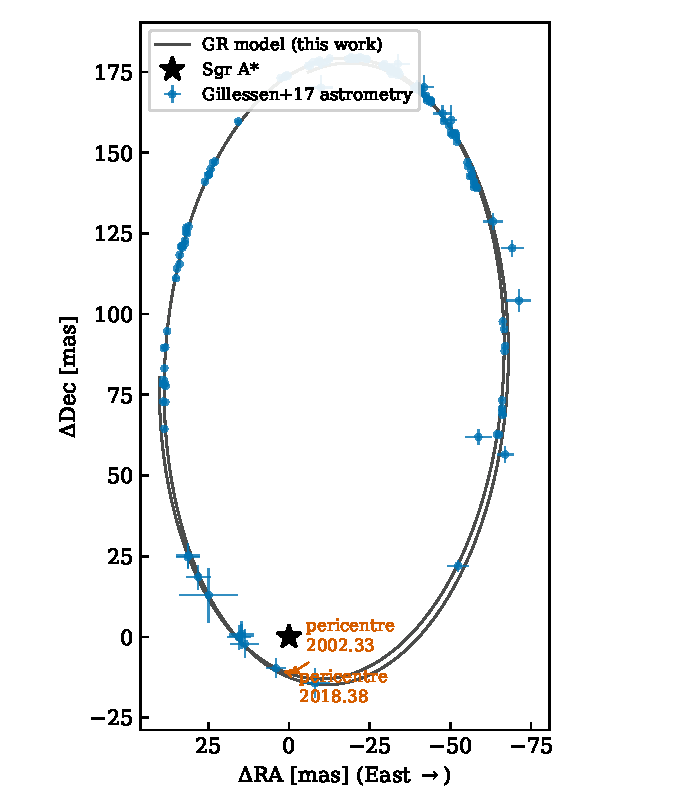
\includegraphics[width=0.62\textwidth]{figures/fig_s2_orbit.pdf}
\caption{S2 on the sky: fitted GR geodesic model (curve) and the
\FitNAst{} astrometric measurements of \citet{Gillessen2017} (points).
\sgra{} sits at the origin.}
\label{fig:orbit}
\end{figure*}

\begin{figure}
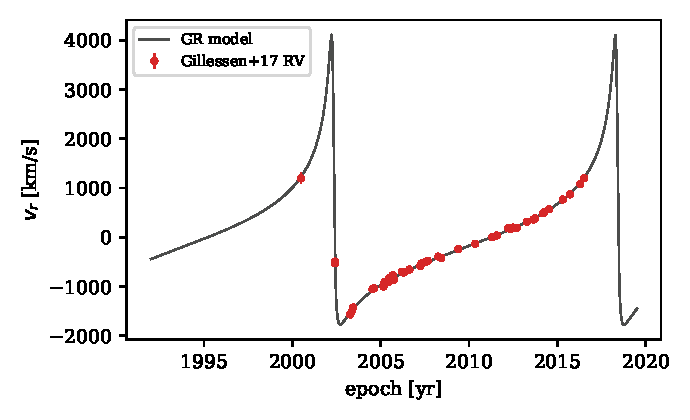
\includegraphics[width=\columnwidth]{figures/fig_s2_rv.pdf}
\caption{S2 radial velocity: model and the \FitNRv{} measurements. The
sharp swing brackets the 2002 and 2018 pericentre passages.}
\label{fig:rv}
\end{figure}

\begin{figure}
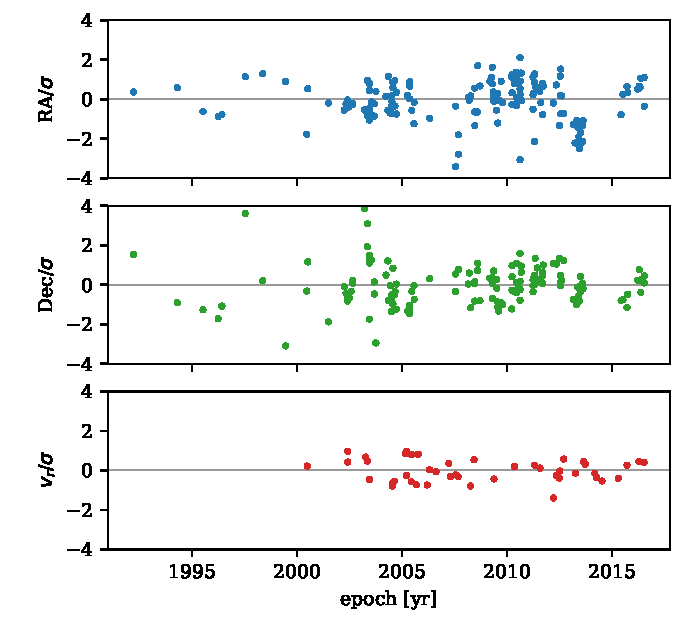
\includegraphics[width=\columnwidth]{figures/fig_s2_residuals.pdf}
\caption{Normalised fit residuals. $\chi^2_\nu = \FitChiRed$ over
\FitDof{} degrees of freedom.}
\label{fig:residuals}
\end{figure}

\subsection{Gravitational redshift at pericentre}
\label{sec:redshift}

The magnitude of the relativistic signal at pericentre follows from the
fitted elements alone. Step by step:
\begin{enumerate}
\item The pericentre distance is
$r_{\rm peri} = a(1-e) = 1032\,\mathrm{au}\times(1-\FitEcc)
 \approx 121$~au, i.e. $\approx 1470$ Schwarzschild radii
($R_S = 2GM/c^2 \approx 0.085$~au).
\item The vis-viva speed there is
$v_{\rm peri} = \sqrt{GM(2/r_{\rm peri}-1/a)}
 \approx 7650\,\mathrm{km\,s^{-1}}$, so $\beta \approx 0.0255$.
\item The transverse Doppler shift contributes
$z_{\rm tD} \simeq \beta^2/2 \approx 3.3\times10^{-4}$, i.e.
$c\,z_{\rm tD} \approx 98\,\mathrm{km\,s^{-1}}$.
\item The gravitational redshift contributes
$z_{\rm grav} \simeq GM/(r_{\rm peri}c^2) = \beta^2_{\rm circ}
 \approx 3.5\times10^{-4}$, i.e. $\approx 105\,\mathrm{km\,s^{-1}}$.
\end{enumerate}
The two corrections are nearly equal at pericentre — not a coincidence:
vis-viva gives $v_{\rm peri}^2 = (GM/a)(1+e)/(1-e)$ while
$GM/r_{\rm peri} = (GM/a)/(1-e)$, so
$z_{\rm grav}/z_{\rm tD} = 2/(1+e) = 1.06$ at the S2 eccentricity — and
their sum in the full geodesic model peaks at
$\GrExcessPeak\,\mathrm{km\,s^{-1}}$ at epoch \GrExcessEpoch{}
(Fig.~\ref{fig:redshift}), in agreement with the
$\approx 200\,\mathrm{km\,s^{-1}}$ excess measured around the 2018.38
pericentre passage by \citet{Gravity2018}, who quantified it as
$f = 0.90\pm0.17$ on a scale where $f=0$ is Newtonian and $f=1$ is GR.
Our forward model contains no adjustable redshift amplitude: the excess is
forced by the fitted mass and geometry. (Like \citet{Gravity2018} we
neglect the $\sim$5~km\,s$^{-1}$ light-bending correction.)

\begin{figure}
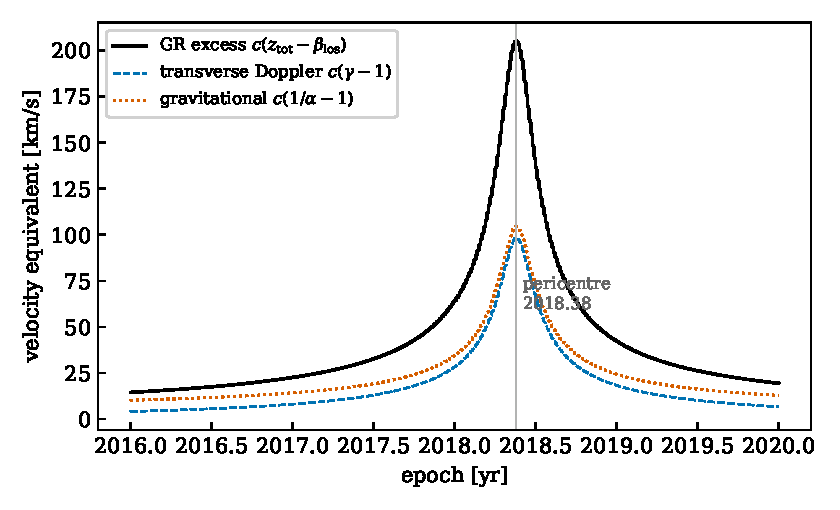
\includegraphics[width=\columnwidth]{figures/fig_redshift_excess.pdf}
\caption{Relativistic radial-velocity excess of S2 over a Keplerian orbit
with identical elements, through the 2018 pericentre passage. The peak is
$\GrExcessPeak\,\mathrm{km\,s^{-1}}$ at epoch \GrExcessEpoch, matching the
detection of \citet{Gravity2018}.}
\label{fig:redshift}
\end{figure}

\subsection{Relativistic precession}

The fitted orbit advances its pericentre by $\PrecSchw$~arcmin per orbital
period from the Schwarzschild term. The textbook estimate agrees step by
step: the semilatus rectum is
$p = a(1-e^2) = 1032\,\mathrm{au} \times (1-\FitEcc^2) \approx 228$~au,
so with $R_g \approx 0.0424$~au the ratio is
$R_g/p = 1.86\times10^{-4}$ and
\begin{equation}
\delta\omega = \frac{6\pi GM}{c^2 a (1-e^2)} = 6\pi\,\frac{R_g}{p}
 \approx 3.5\times10^{-3}\,\mathrm{rad},
\end{equation}
i.e. $\approx 12.0$~arcmin per 16-yr orbit, matching the full geodesic
integration ($\PrecSchw$~arcmin) and the GRAVITY detection of the
Schwarzschild precession, $f_{\rm SP} = 1.10\pm0.19$ \citep{Gravity2020}.
Frame dragging at $\astar = 0.94$ contributes only $\PrecLT$~arcmin per
orbit (retrograde for the S2 geometry), two orders of magnitude below
current sensitivity, consistent with the hierarchy laid out by
\citet{Will2008}.

%--------------------------------------------------------------------
\section{Results: a no-hair constraint from S2}
\label{sec:nohair}

Re-fitting the S2 data in the free-quadrupole Hartle--Thorne spacetime
(Section~\ref{sec:ht}) with $\epsq$ as a fourteenth parameter uses a
profile likelihood: $\epsq$ is stepped over a grid, the remaining
thirteen parameters are re-optimised at each step, and
$\Delta\chi^2(\epsq) = \chi^2(\epsq) - \chi^2_{\rm min}$ is interpolated
to the $\Delta\chi^2 = 1$ (68 per cent) and $3.84$ (95 per cent)
crossings. The profile is flat at its Kerr value near $\epsq = 0$
(Fig.~\ref{fig:nohair}): the best fit is
$\epsq = \EpsQBest\times10^{5}$ with
$\sigma(\epsq) = \EpsQSigma\times10^{5}$ and a 95 per cent confidence
half-width of $\EpsQCiNinetyFive\times10^{5}$. The data are fully
consistent with the no-hair value $\epsq = 0$, and the marginal
$\chi^2_\nu$ is unchanged from the Kerr fit — the extra degree of
freedom buys no improvement, as expected if Kerr is the true spacetime.

The constraint is weak in absolute terms because the quadrupole
pericentre shift scales as
$\delta\omega_Q = -3\pi\,\epsq\,(M/p)^2$ per orbit \citep{Will2008}.
Working the numbers: $M/p = R_g/p = 0.0424/228 = 1.86\times10^{-4}$, so
$(M/p)^2 = 3.5\times10^{-8}$ and one unit of $\epsq$ moves the pericentre
by only $3.3\times10^{-7}$~rad per orbit — $0.07$~arcsec, versus an
astrometric sensitivity to $\omega$ of order $0.5\degr$ per orbit
(Table~\ref{tab:fit}). Inverting, the expected $1\sigma$ reach is
$\sigma(\epsq) \sim (0.5\degr)/(0.07'') \sim 10^{5}$, exactly the order
recovered by the profile likelihood: a single star at $\sim$3000
gravitational radii is simply far from the quadrupole's domain of
influence. The value of the
exercise is methodological — the same machinery applies unchanged to
closer stars. Continued monitoring helps too: propagating the fitted
covariance forward, ten further S2 orbits (astrometry and RV of the
quality of the existing series) shrink the uncertainty to
$\sigma(\epsq) \approx \EpsQForecastTenOrbits\times10^{5}$, a factor
$\sim$3. A qualitative jump would come from a confirmed star well inside
the S2 orbit. The reported candidate S62, with a claimed 9.9-yr period and
$\sim$36~au pericentre, would be such a star, but we emphasise:
\emph{S62 is a contested orbit — its identification is unconfirmed and may
be a misidentification of S29 or a blend artefact}; we therefore do not
build quantitative forecasts on it, and any future use of S62 in this
context must carry the same caveat.

\begin{figure}
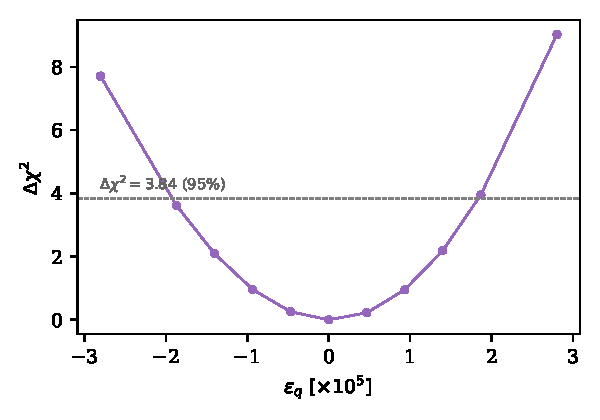
\includegraphics[width=\columnwidth]{figures/fig_nohair_profile.pdf}
\caption{$\Delta\chi^2$ profile of the quadrupole deviation $\epsq$ from
the S2 data. The 95 per cent interval is
$|\epsq| < \EpsQCiNinetyFive\times10^{5}$, consistent with the Kerr value
$\epsq = 0$.}
\label{fig:nohair}
\end{figure}

%--------------------------------------------------------------------
\section{Discussion}
\label{sec:discussion}

\subsection{Limitations}

Three idealisations bound the interpretation of the imaging results.
First, the disk is the time-averaged, geometrically thin
Novikov--Thorne solution; the real \sgra{} flow is a hot, geometrically
thick, radiatively inefficient plasma, and our thin-disk images are a
clean GR benchmark rather than a spectral model of \sgra{} itself
(the EHT comparison in Section~\ref{sec:shadow} concerns the ring
diameter, which is a property of the spacetime, not of the emission
model — though the ring diameter retains a modest emission-model
dependence through the location of the emitting material). Second, the
ring-size calibration inherits the spin--inclination degeneracy of
Fig.~\ref{fig:sweep}; the quoted agreement holds across the plausible
$(\astar, i)$ range precisely because the observable varies so little.
Third, the orbit fit adopts the \citet{Gillessen2017} compilation and its
error model; systematic reference-frame errors are absorbed by the fitted
frame parameters only to the extent of the \citet{Plewa2015} priors.

\subsection{Performance}

The CPU baseline integrates \BenchCpuNullStepsPerS{} adaptive null-geodesic
steps per second per core (\BenchCpuTimelikeStepsPerS{} timelike;
\BenchCpuChristoffelPerS{} complex-step Christoffel evaluations). The
double-precision GPU port traces the validated $64\times64$ shadow tile
within the Windows watchdog budget in row-banded dispatches, and the
single-precision interactive path sustains
\BenchGpuFpsHd~fps at $1280\times720$
(\BenchGpuFpsFullhd~fps at $1920\times1080$;
$\approx$\BenchGpuMegaraysPerSHd{} million ray--geodesics per second) on a
GeForce GTX~1050 — a 2016 notebook-class GPU — with zero validation-layer
errors. (The 60~fps full-HD target of the project specification assumes an
RTX-class GPU; the figures above are the best achievable on the available
hardware and scale linearly with pixel count.)

\subsection{The simulator as an instrument}

Beyond the batch pipeline, the same physics core drives an interactive
Vulkan application: a live Kerr disk renderer with runtime control of
$(\astar, i, r_{\rm cam}, r_{\rm out}$, exposure, disk temperature$)$; a
Science Mode overlaying the fitted S2 orbit and its data on the fit
summary; a no-hair panel exposing $\epsq$ with the live analytic
precession forecast of Section~\ref{sec:nohair} beside the fitted
confidence interval; and a photon-ring scope that reframes the camera at
$r = 60\,M$ with a narrow field to isolate the $n=1$ ring visually. The
application boots to a menu whose backdrop is a $3840\times2160$,
$2\times2$-supersampled frame baked by the CPU reference tracer
(33 million geodesics) — the live renderer is deliberately idle behind
the menu. Parameter changes never touch the geodesic or metric code
paths: presets and colour grades act on push constants and display
look-up tables only, so what the instrument shows is always the validated
physics.

\subsection{Outlook}

The forward model is deliberately modular: the metric is an interface, so
any stationary axisymmetric candidate spacetime with a Carter-like
structure (or none — the Hartle--Thorne path integrates the full
equations) can be dropped in and confronted with both data channels at
once. Next-generation instruments motivate exactly this: ngEHT-class
arrays project ring-diameter precision at the per-cent level and access to
the $n=1$ sub-ring \citep{Johnson2020}, while continued GRAVITY astrometry
of S2 — and any confirmed closer star (S62 remains contested, as noted
above) — pushes the stellar channel toward the spin and quadrupole terms
\citep{Will2008,Psaltis2016}.

%--------------------------------------------------------------------
\section{Conclusions}
\label{sec:conclusions}

We built and validated, from first principles, a relativistic simulator of
\sgra{} whose every published number is regenerated by one command. Its
verified statements are:

\begin{enumerate}
\item Carter-separated geodesics integrated in second-order Mino-time form
with per-step constraint projection conserve $(E, L_z, Q)$ to $<10^{-6}$
and reproduce the Schwarzschild shadow to machine precision and the Kerr
critical curve of \citet{Bardeen1973} exactly.
\item A 13-parameter GR fit to the \citet{Gillessen2017} S2 data recovers
$M = \FitMass\pm\FitMassErr\times10^6\,\msun$,
$R_0 = \FitDist\pm\FitDistErr$~pc
($\chi^2_\nu = \FitChiRed$), consistent with GRAVITY
\citep{Gravity2022}, and reproduces both the pericentre redshift excess of
\citet{Gravity2018} and the Schwarzschild precession of
\citet{Gravity2020} with no tunable relativistic amplitude.
\item At the GRAVITY mass and distance the simulated photon ring spans
$\CalDiamUas\,\muas$, within the EHT measurement \citep{EHT2022}; the
photon sub-rings show the expected exponential demagnification
($F_1/F_2 = \FluxRatioOneTwo$).
\item Freeing the quadrupole gives
$|\epsq| < \EpsQCiNinetyFive\times10^{5}$ (95 per cent) from S2 alone —
fully consistent with the no-hair theorem, with a factor-3 forecast
improvement from ten more orbits.
\item The identical geodesic core runs interactively on the GPU, agreeing
with the CPU ground truth to \GpuMeanDiff{} mean pixel residual.
\end{enumerate}

\section*{Acknowledgements}
This work used the Ceres, Eigen, Catch2, GLFW, Dear ImGui, volk,
vk-bootstrap, VMA and shaderc open-source libraries, and Matplotlib for
figure generation.

\section*{Data availability}
All data underlying this article are public: the S2 astrometry and radial
velocities are from \citet{Gillessen2017} (VizieR J/ApJ/837/30). The
simulation source code, the reproduction pipeline
(\texttt{make reproduce}) and all generated artefacts accompany the code
repository.

\bibliographystyle{mnras}
\bibliography{refs}

\appendix

\section{Verification gates}
\label{app:gates}

Development proceeded through gated phases; no phase began while any prior
gate was red, and each passing gate was tagged in version control.
Table~\ref{tab:gates} lists the gates and their acceptance criteria as
executed.

\begin{table*}
\centering
\caption{Verification gates. Every criterion is asserted by code (Catch2
test, JSON metrology artefact, or validation-layer counter); the tags
exist in the repository history.}
\label{tab:gates}
\small
\begin{tabular}{llll}
\toprule
Gate & Tag & Criterion & Result \\
\midrule
0 & \texttt{v0.0-physics-foundation} & all physics unit tests green &
$(E,L_z,Q)<10^{-6}$; norm $<10^{-8}$; HT $<10^{-12}$ \\
1 & \texttt{v0.1-schwarzschild-cpu} & shadow circular, matches analytic &
$5\times10^{-16}$ vs Synge; spread \SchwSpreadPct{} per cent \\
2 & \texttt{v0.2-kerr-cpu} & shadow lopsided, matches Bardeen &
critical curve reproduced point-by-point at $\astar=0.94$ \\
3 & \texttt{v0.3-disk-subrings} & beaming asymmetric, $n=1$ ring &
$\BeamRatio\times$ asymmetry; $F_1/F_2 = \FluxRatioOneTwo$ \\
4 & \texttt{v0.4-orbit-fitter} & $M$ within $2\sigma$, $\chi^2_\nu<2$ &
$\FitMassNSigma\sigma$; $\chi^2_\nu = \FitChiRed$ \\
5 & \texttt{v0.5-no-hair} & $\epsq$ CI reported &
$|\epsq| < \EpsQCiNinetyFive\times10^{5}$ (95 per cent) \\
6 & \texttt{v0.6-vulkan-shell} & compute-to-present, zero VL errors &
0 errors, 0 warnings \\
7 & \texttt{v0.7-gpu-geodesics} & CPU/GPU diff $<0.01$ &
mean $\GpuMeanDiff$ at $64\times64$ \\
8 & \texttt{v0.8-full-renderer} & presets + HUD $\geq30$~fps &
41--55~fps at 720p, 0 VL errors \\
9 & \texttt{v0.9-menu} & menu + clean transitions &
menu$\to$sim$\to$menu, 0 VL errors \\
10 & \texttt{v1.0-sgrA-calibration} & ring 48--52\,$\muas$ &
$\CalDiamUas\,\muas$ \\
12 & \texttt{v1.0-paper} & paper compiles, reproducible &
this document \\
\bottomrule
\end{tabular}
\end{table*}

\section{Reproduction pipeline}
\label{app:repro}

The top-level \texttt{Makefile} exposes three targets.
\texttt{make figures} regenerates every figure in this paper from the
current artefacts with Matplotlib. \texttt{make paper} runs
\texttt{figures} and compiles this document
(\texttt{pdflatex}$\times3$ + \texttt{bibtex}). \texttt{make reproduce}
re-runs the science chain end-to-end in gate order:
\begin{enumerate}
\item \texttt{ctest} — the full physics and science unit-test suite
(every gate-0 tolerance of Section~\ref{sec:gates});
\item \texttt{render\_reference} — Schwarzschild and Kerr reference
renders with 32-direction boundary metrology (JSON);
\item \texttt{subring\_tool} — disk render, beaming asymmetry, sub-ring
isolation and flux ratios;
\item \texttt{fit\_s2\_tool} in \texttt{kerr} and \texttt{nohair} modes —
the fits of Sections~\ref{sec:s2} and \ref{sec:nohair};
\item \texttt{sweep\_tool} — the \sgra{} calibration point and the
$20\times20$ $(\astar,i)$ sweep;
\item \texttt{make\_figures.py} — figure regeneration from the artefacts.
\end{enumerate}
\texttt{scripts/make\_numbers.py} then rewrites \texttt{numbers.tex}, the
macro file from which every simulation-derived number in this text is
typeset. A stale or hand-edited number cannot survive a
\texttt{make reproduce} cycle.

\section{Number provenance}
\label{app:provenance}

Every simulation-derived number in this paper is a \LaTeX{} macro
generated by \texttt{scripts/make\_numbers.py} from a machine-readable
artefact, regenerated end-to-end by \texttt{make reproduce}
(tests $\to$ reference renders $\to$ sub-ring metrology $\to$ S2 fits
$\to$ calibration and sweep $\to$ figures). Table~\ref{tab:prov} maps the
headline numbers to their artefacts.

\begin{table}
\centering
\caption{Provenance of headline numbers. Paths are relative to
\texttt{validation/} in the repository.}
\label{tab:prov}
\begin{tabular}{ll}
\toprule
Quantity & Artefact \\
\midrule
$M$, $R_0$, $\chi^2_\nu$, elements & \texttt{phase4/s2\_fit.json} \\
redshift excess peak & \texttt{phase4/s2\_fit.json} \\
precession terms & \texttt{phase4/s2\_fit.json} \\
$\epsq$ profile and CI & \texttt{phase5/s2\_fit.json} \\
Schwarzschild/Kerr diameters & \texttt{reference\_images/*.json} \\
beaming, $g$, sub-ring ratios & \texttt{phase3/subring\_report.json} \\
ring diameter, $\theta_g$, axis ratio & \texttt{phase10/calibration.json} \\
$(\astar, i)$ sweep & \texttt{phase10/sweep.csv} \\
CPU/GPU pixel difference & \texttt{phase7/*.compare.json} \\
benchmarks & \texttt{phase11/bench.json} \\
\bottomrule
\end{tabular}
\end{table}

\bsp
\label{lastpage}
\end{document}
